\section{Anonymisering av bilder med ansikter}
\subsection{Bakgrunn}
Anonymisering av bilder er enkelte ganger nødvendig før det blir offentlig vist frem for å skjerme den avbildedes personvern. En teknikk som ofte blir brukt er å gjøre ansiktene uskarpe og resten av bildet forblir skarpt. Teknikken avhenger av at programmet klarer å gjenkjenne ansiktene\cite{wiki:FaceDetection} for å definere en maske rundt, slik at man kan isolere anvendingen av bildet kun på ansiktet, og i likhet som tidligere er det flere teknikker som benyttes. I denne oppgaven brukte vi biblioteket OpenCV\cite{cv2} (Open Source Computer Vision Library) og maskinlæringsalgoritmen Haar Cascade\cite{haar}. 



\subsection{Open CV}
Open CV er et open source datasyn-\footnote{Computer Vision\cite{datasyn}} og maskinlæringsbibliotek som ifølge dem selv\cite{cv2} ble utviklet for å skape et felles infrastruktur for datasynsapplikasjoner og for å akselerere bruken av maskinoppfatning\footnote{Machine perception\cite{wiki:machinePerception}} i kommersielle produkter. Kort fortalt betyr dette datamaskinens evne til å tolke data på en måte som ligner på måten mennesker bruker sansene til å oppfatte3 verden rundt seg\cite{wiki:machinePerception}, og da spesielt synet i dette tilfellet.  
\subsection{Haar Cascade}




%\import{./kode/}{anonymiseringModul}
%\begin{center}
%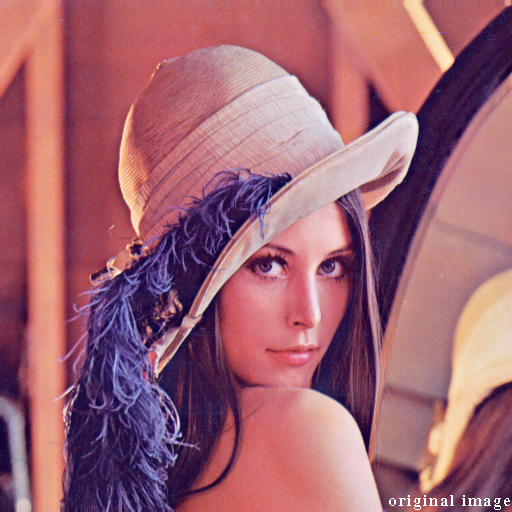
\includegraphics[scale = 0.3]{./bilder/Anonyme/lena.png}
%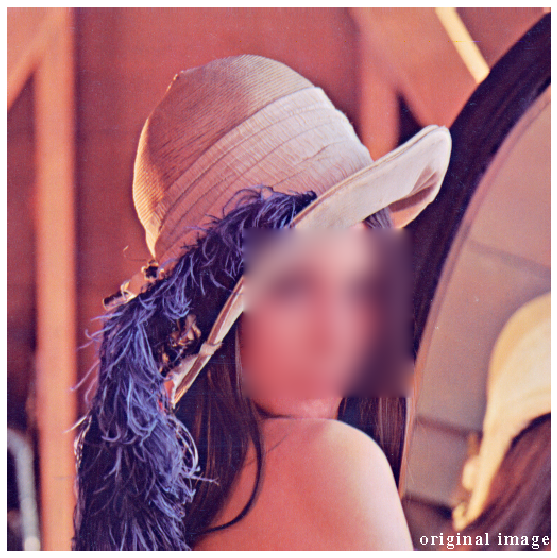
\includegraphics[scale = 0.28]{./bilder/Anonyme/lenaBlur.png}
%\end{center}